% !TeX root = ../main.tex
% Add the above to each chapter to make compiling the PDF easier in some editors.

\chapter{Methodology}\label{chapter:methodology}

\section{Terminology}\label{sec:terminology}

Before we dive into technical explanations, we want to clear some potential terminology confusion.

In the original DICE release from Microsoft~\cite{England2016}, the identifier of a component is called the \ac{FWID}.
The \ac{TCG} consortium later renamed it \ac{TCI}.
We believe this is to emphasize that the TCI does not necessarily have to be the hash of a firmware binary, but could also be, for example, the embedded ID of a hardware component.
However, \ac{TCG} has not fully adopted this terminology renaming.
Their DICE Attestation Architecture~\cite{TCGAttestation2021} defines an X.509 extension that contains the \acp{TCI}.
They continue to be referred to as \acp{FWID} in the machine-readable formal definition of this extension, while everywhere else they are referred to as \acp{TCI}.
In personal correspondence with \ac{TCG}, we have learned that this is due to backwards compatibility.
The old term \ac{FWID} is retained whenever it is used in something that is alive in the long term, like formal definitions, and the new term \ac{TCI} in assets that can be updated more quickly, such as the specification text.
Therefore, we will use the term \ac{TCI} in this theoretical chapter, and in the implementation chapter (\autoref{chapter:implementation}) we will use the term \ac{FWID}, just as it is common practice at the \ac{TCG}\@.
This ensures that the explanation of our implementation better matches the actual code, where \ac{FWID} is the term as it is used by automatically generated code.

Occasionally, the name of an asymmetric key is suffixed with `priv', `pub' or `cert' to designate the private part, the public part, or the certificate, respectively.
For example, EKpriv refers to the private portion of EK\@.
And EKcert corresponds to the certificate with EKpub as its subject key.

% Prover/Verifier (in many earlier papers) vs. Attester/Verifier/Relying Party (RFC)


\section{Architectural overview}\label{sec:arch_overview}

\begin{figure}[htpb]
  \centering
  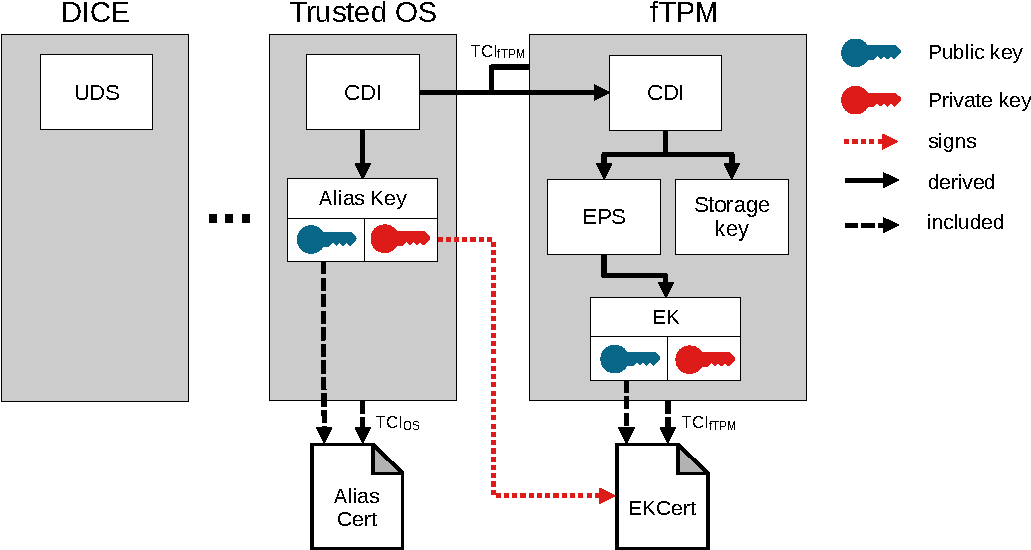
\includegraphics[width=1\linewidth]{figures/architecture.pdf}
  \caption{The architecture of our system.} \label{fig:architecture}
\end{figure}


The architecture of our proposed and later implemented system is illustrated in \autoref{fig:architecture}.
As you might notice, it is similar to our overview picture of \ac{DICE} (\autoref{fig:dice-layers}).
This is to be expected, since our system leverages \ac{DICE} as our \ac{SRTM}.
Static in this context means that it uses the trusted state that a device has at the always same point in time, here after switching on, for further measurements.
This is in contrast to a \ac{DRTM}, which is able to do this at any time, e.g., Intel SGX\@.

The boot process continues from here in the usual \ac{DICE} manner until the firmware TPM is reached.
The component that measures the \ac{fTPM} is usually the trusted operating system running in EL1 in the secure world, as seen in \autoref{fig:arm_trustzone_arch}.
Like any other \ac{DICE} component, the \ac{fTPM} receives its secret \ac{CDI} from its predecessor layer.
Recall that the \ac{CDI} is tied to the identity of the \ac{fTPM} including the entire underlying firmware stack and the \ac{UDS}\@.
We derive two values from the \ac{CDI}\@.

\subsection{Storage key}

% Storage Key generation

While the trusted OS within the \ac{TEE} might already encrypt data before it is sent to the storage device, this only binds the data to the \ac{TEE}, but not the identity to the \ac{fTPM}.
For this purpose, we first derive a storage key from the \ac{CDI}.
This is a symmetric encryption key that is used to encrypt the \ac{fTPM} storage space in RAM before it is written to a persistent storage space such as a hard disk drive~(HDD).
At no time does the HDD see plaintext data (\autoref{fig:storage-encryption}).
As the storage key is derived from the \ac{CDI}, the storage data is only accessible to the \ac{fTPM} with the exact identity with which it was generated.
For example, its identity changes due to a \ac{TPM} modification or an update of a previous firmware component, which results in a full manufacturer reset of the fTPM\@.
This enables the property that an \ac{fTPM} storage must never be accessible to another \ac{TPM}\@.

\begin{figure}[htpb]
  \centering
  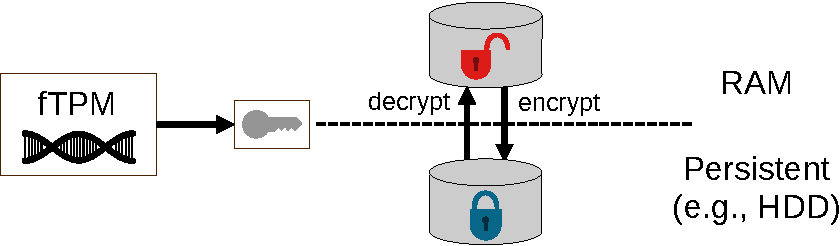
\includegraphics[width=0.8\linewidth]{figures/storage-encryption.pdf}
  \caption{The fTPMs' storage is protected by a key derived from its identity.} \label{fig:storage-encryption}
\end{figure}


An attacker could thereby easily trigger a data loss.
This must be avoided by integrating good-practices with working with a \ac{TPM}, which includes having secrets stored also elsewhere.
Microsoft recommends backing up all secrets stored on the \ac{TPM} before clearing it~\cite{MicrosoftClearRecommendations}, what can be generalized to the backup of the fTPM data in all cases where data loss causes serious damage.

% For pure data or fTPM rollback: RPMB reduces possible attackers to components in the TEE. No entire protection.
% But for data protection by downgrading the fTPM: Our solution is more secure than only using RPMB, see paragraph below. In short, we do not need to trust entire software stack in TEE.

Establishing the storage key also prevents an attacker from accessing an fTPM's data by downgrading the fTPM\@.
For example, if an attacker wants to access data stored in a particular fTPM and can exploit a vulnerability of an earlier version of that fTPM, it is not possible to replace the fTPM with its old version, as neither the attacker nor the fTPM itself will be able to decrypt the previous data.

However, it does not protect against the isolated downgrade of the fTPM itself or solely its data.
When the fTPM is downgraded, as previously described, the data is reset.
Nevertheless, new data generated by the downgraded TPM might still be leakable by vulnerabilities of the downgraded fTPM\@.
Our storage key also does not protect the fTPM data from a rollback attack, i.e., the freshness of the fTPM data is not guaranteed.
This attack can be attractive for malicious actors to reset the try count of PINs to work around the lockout mechanism of the TPM\@.
Another example is to restore the data wherein a secret was stored, however, not yet protected by a PIN\@.
% A malicious actor requires the TPM to decrypt the data, as it is encrypted.
The protection against the rollback of fTPM data or the fTPM itself can be achieved by storing them in a Replay Protected Memory Block~(RPMB) partition~\cite{eMMC, UFS}.
For this reason, an RPMB partition is part of Microsoft's hardware requirements for a firmware TPM~\cite{Raj2015}.

Only the TEE can write to the RPMB (authenticated write).
And the TEE can ensure that received data really originates from the RPMB (authenticated read).
Each command is unique due to a nonce (for read operations) or a write counter (for write operations), which prevents replay attacks.
The secure channel to the RPMB is established by a secret key shared between the TEE and the RPMB\@.
Hence, every component within the TEE can arbitrarily access and modify the data on the RPMB, and must therefore be trusted.
This is different to our approach with the storage key, whereby we bind the access to the data to the identity of the fTPM, i.e., we trust only the identity of the fTPM instead of the entire TEE\@.
In other words, we seal the data of the fTPM with the identity of the fTPM instead of allowing the entire TEE to access the data at any time.
However, RPMB and our storage key are orthogonal and can be used in conjunction.

% , as each component in the TEE can read from or write to the RPMB partition arbitrarily.
% This is independent of the component's identities.
% In our approach with the storage key, the fTPM does not have to trust its preceding components, because as soon as one of them changes, the fTPM itself no longer has access to the data.

% Indeed, the fTPM itself can also be stored in a RPMB partition, which builds another rollback protection aside of our approach with the storage key.
% However, this protects the data on different levels.
% The encryption with our storage key introduces confidentiality and integrity of the fTPM's data sealed to the identity of the fTPM\@.
% RPMB protects the data's confidentiality, integrity and freshness from access outside the TEE, assuming the RPMB is only accessible from the TEE, which is the typical design.
% Hence, while the RPMB protects additionally freshness, we bind our security guarantees tighter to the exact identity of the fTPM instead of merely to the specific TEE\@.

% So, our mechanism additionally protects data-at-rest, while the data-at-use is protected by the TEE's secure memory, i.e., the memory isolation from the normal world.

\subsection{EPS and EK}

% EPS Generation

Then, the \ac{EPS} is generated based on the \ac{CDI}\@.
It is the seed that is used to generate the primary \ac{EK}.
A primary key in the sense of the TPM means that it has no parent key, but a parent seed, here the \ac{EPS}\@.
The indirection of generating the \ac{EK} from the \ac{EPS} via the \ac{CDI} instead of generating it directly from the \ac{CDI} is introduced because the code of fTPMs can be hardcoded to use the \ac{EPS} during \ac{EK} generation.
And we want our system to require as few modifications to TPM code as possible.
The \ac{CDI} must also be removed from memory as quickly as possible to reduce the time frame in which leaks are possible, but the \ac{EPS} must be accessible to the \ac{fTPM} throughout its entire runtime.
It is therefore good practice to extract long-term secrets from the short-term secret \ac{CDI} and then quickly delete the \ac{CDI} from memory.

% Device identification

The \ac{EK} of a dedicated TPM represents the long-term identity of its host device as long as the TPM is not soldered or plugged away.
Our \ac{EK} does not do this because a firmware TPM is software-based and changes every time the fTPM or the underlying firmware is modified, without the host device changing.
Instead, we use the DICE for this, which is hardware-based.
Its DeviceID key, as the name suggests, represents the device identity.
Note that the DeviceID contains the identity of layer 0 of the boot chain, i.e., the first mutable code.
This can also be seen in \autoref{eq:dice_deviceID}.
For this reason, the DICE specification suggests keeping the first mutable code as small as possible so that it remains constant throughout the life of the device~\cite{dice-layering-arch}.

% EK is a signing key

By default, the \ac{EK} is a restricted encryption key.
It is not used for signing by default because the resulting signatures may reveal the TPM's identity.
We deviate from that by creating the \ac{EK} as a restricted signing key.
While this breaks privacy of the prover, it has the advantage of not requiring a third party \ac{CA}\@.
More details and an extension to our system introducing privacy is provided in \autoref{sec:privacy}.

\section{The identity of a firmware TPM}

DICE offers two identities for each component---the TCI and the CDI\@.
As shown in \autoref{eq:dice_cdi}, the CDI of a component changes when (i) the identity of the hardware changes, i.e., the \ac{UDS}, (ii) the identity of a preceding component changes, or (iii) the component itself changes.
In contrast, the TCI is the identity of a single component, considered in isolation, usually the hash of its binary, i.e., only for case (iii).
% It only changes when the component itself is changed, regardless of the hardware or preceding components.
So, while a CDI should be statistically unique since it is derived from a \ac{UDS} with this property, a given TCI can be found on many devices if they contain exactly the same software component.
Note that a component's TCI is part of its CDI, as shown in \autoref{fig:identities}.

\begin{figure}[htpb]
  \centering
  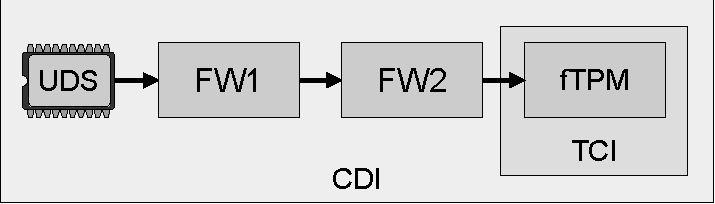
\includegraphics[width=0.6\linewidth]{figures/identities.pdf}
  \caption{Visualizing the difference between the CDI and the TCI from the perspective of an fTPM component. The identity of the hardware is provided in the form of the UDS.} \label{fig:identities}
\end{figure}


Hence, we decided to derive the identity of an fTPM, i.e., its \ac{EK}, ultimately from the CDI\@.
This binds the identity of the fTPM to any security-relevant component preceding it.
The rationale for this is that once a previous component has changed, it is unknown whether it has gone into a benign or malicious state.
And if it is malicious, it could change the firmware TPM and thereby access its sensitive material such as private keys.
Although this is later recognized by the verifier during remote attestation, sensitive data could still be leaked.
If the identity of the firmware TPM is extended to everything prior to the fTPM, its data is no longer accessible as soon as something preceding it changes.
This is due to the derivation of the storage key from the CDI\@.
And this behavior should also be reflected in the EK, so that the storage key and the EK should always change together or not change at all.

The TPM's storage cannot be part of its identity as it changes during runtime after each data write, e.g., storing an arbitrary key.
This is a problem because DICE only runs during the boot time in which the identity of the fTPM is measured.
The identity of the fTPM must not change afterwards, otherwise the identity reported by DICE and the actual identity of the fTPM would be inconsistent.
We also do not want to restrict the permissible values of the working data of an fTPM, which makes its measurement as part of the TCI pointless.

% Depending on the point of view, there are two identities of an fTPM, as shown in \autoref{fig:identities}.
% There is the identity of the fTPM measured by DICE, which consists of the hash of the binary and the component configurations as for all DICE components, as shown in \autoref{fig:ftpm-identity}.
% This identity is referred to as the TCI.
% Compilation flags are not part of these configurations, as they are embedded in the final binary and are therefore automatically measured as part of the measurement of the binary.
% Of more interest are the configurations that are not part of the binary.
% They are usually provided in well-known formats such as \texttt{json} or \texttt{xml}.
% However, Microsoft's fTPM reference implementation does not contain such configurations, which simplifies the TCI generation of our fTPM by limiting it to the measurement of the fTPM binary data.
% The TPM's storage cannot be part of its identity as it changes during runtime after each data write, e.g., storing an arbitrary key.
% This is a problem because DICE only runs during the boot time in which the identity of the fTPM is measured.
% The identity of the fTPM must not change afterwards, otherwise the consistency of the identity transmitted by DICE and the actual identity of the fTPM would differ.
% We also do not want to restrict the permissible values of the working data of an fTPM.
% In summary, the CDI keeps being updated from layer to layer, the TCI is calculated for each layer individually.
% Then, there is also the identity of the fTPM in the TPM context, which is represented by its EK.
% This identity is not only bound to the binary and the configuration of the fTPM, but also the entire underlying firmware stack.
% We derive the EK from the TPMs CDI, which is derived of the measurements of all preceding firmware components and the TPM's TCI, see \autoref{eq:dice_cdi}.

% \begin{figure}[htpb]
  \centering
  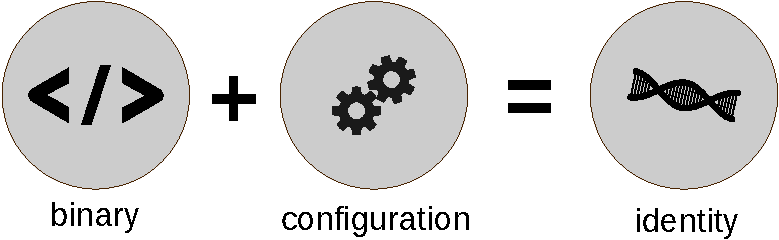
\includegraphics[width=0.6\linewidth]{figures/ftpm-identity.pdf}
  \caption{The accumulation of the binary and its configuration to its identity.} \label{fig:ftpm-identity}
\end{figure}


% Configurations required
% Does contain whole firmware stack?
% Data cannot be considered, since changes during runtime, not represented by DICE which only happens at boot-time
% What happens if identity changed? -> Data not accessible, in essence, fTPM fully reset
% https://trustedfirmware-a.readthedocs.io/en/latest/design_documents/measured_boot.html#critical-data

% \section{Provisioning process}

% To summarize, attestation key provisioning must ensure that only valid attestation key material is established in Attesters [RFC 9334]

\section{Attestation process}\label{sec:attestation_process}

% Check also for revocation of manufacturer cert

% We use explicit attestation. See DICE Layering Spec 7.2
% See 8.1.1.2 for an example about implicit attestation
% Implicit attestation would require to know all resulting public keys in EKcert, which would require that we booted it up in a controlled manner beforehand and stored the resulting code.
We use an explicit attestation procedure.
This makes it sufficient for the verifier to know its trusted TCIs, whereas implicit attestation would require a database of trusted Alias public keys representing a trusted component.
And since each Alias public key is device unique, as it roots in the device's unique \ac{UDS}, the verifier would need to know all alias public keys for each component on every device declared trustworthy, which we consider unrealistic.
Also, this would be a hindrance as the verifier should be able to establish trust into an unknown device by trusting the DICE manufacturer, and knowing the identities of trustworthy firmware.

% Secure channel must be established by requiring communication with the private key corresponding to the public key in the EKcert.
% This allows a verifier to validate that the prover is in posession of the private key, and hence, the included identities in the certificate chain are trustworthy.

\subsection{Verifier establishes trust to the prover's fTPM}\label{subsec:trust_prover_tpm}

% It is exactly the purpose of our system to make this possible for the verifier.
First, the verifier retrieves the DICE certificate chain generated by our solution from the prover.
After verifying that the signatures of the certificate chain are valid, the verifier checks whether the DICE implementation is trustworthy by knowing its manufacturer.
This also involves checking if the DeviceID certificate issued by the manufacturer was revoked.
Such an event might occur if the security of an old DICE implementation is broken, and the manufacturer wants to reflect this.

At this point, the verifier must traverse the certificate chain starting from the root and verify whether each component represented by a certificate is trusted, by checking the embedded TCI\@.
An untrusted component must be assumed to lie about its conducted measurements.
For example, it can modify the subsequent component without reflecting this in the measurement of the TCI\@.
Consequently, as soon as a component is untrusted, all subsequent components have to be considered untrusted as well.
This behavior is also represented mathematically in \autoref{eq:dice_attestation}.
Therefore, trusting the fTPM requires to trust all underlying firmware components.
\begin{equation}
    \label{eq:dice_attestation}
    C_{i, \, trusted} \, \coloneqq \, \bigwedge_{k=0}^{i} trusted(C_{k})
\end{equation}

% \subsubsection{Example security policies for a component}

The \(trusted\) function of \autoref{eq:dice_attestation} checks the information provided by a certificate~\(C\) against security policies defined by the verifier.
In the following, we would like to present some example policies for improving comprehensibility for the reader.

\begin{itemize}
    \item We generally do not trust the component's manufacturer and therefore, do not trust the component.
    \item The component is up-to-date, and there are no known vulnerabilities and therefore, we trust the component.
    \item The component is outdated, but all updates are only functional instead of security-relevant, so we still trust it.
    \item We do not know the TCI of the component. We follow a `Deny by default' policy. Therefore, we do not trust the component.
\end{itemize}

After doing all this, the verifier can only state that ``I trust the certificate chain and the components of \emph{some} machine represented by it.''
This is due to the possibility of any actor to simply replay the certificate chain.
But we need to promote the \emph{some} to \emph{the machine I communicate with}.
This is solved in subsequent protocols where the prover is challenged to be in control of EKpriv which corresponds to the EKpub of the EK certificate.
For example, by verifiying the subsequently retrieved quote.
Although this is not explicitly part of our proposed solution, we nevertheless describe it for better understanding and provide a comprehensive explanation of the entire attestation process.

\subsection{Verifier establishes trust to the prover's quote}\label{subsec:trust_quote_from_prover}

For that, the verifier needs to know that the quote was signed with the restricted EKpriv corresponding to the EKpub in EKcert, and that the fTPM is in control of EKpriv.
The verifier also needs to trust that the fTPM did not leak EKpriv, as this would not only allow to replay a whole certificate chain, but even succeed the subsequent protocols with the leaked EKpriv.
The verifier can derive whether it considers the EKpriv of the fTPM as not leaked based on the fTPM's TCI value, as one requirement of trusting a TCI must be whether the verifier considers the component to keep its security guarantees.

To trigger the protocol, the verifier sends a nonce to the prover, which includes it in the quote request sent to the firmware TPM, i.e., \texttt{TPM2\_Quote}.
The nonce prevents replay attacks.
The verifier also needs to know that the EK is restricted.
Otherwise, a compromised prover could generate quotes representing arbitrary states which do not represent the prover's actual state.

Usually, this is ensured by manufacturers in that they only sign an EKcert for a restricted EK\@.
Of course, this cannot be applied to our solution, as our EKcert is dynamically created without a TPM manufacturer asserting specific attributes of the EK\@.
Instead, the verifier needs to derive from the fTPM's TCI embedded in the EKcert that the EK is restricted.
For the EK's attributes to be represented in the TCI, the template containing the EK's attributes must be generated in the firmware TPM's code.
This ensures that the TCI also represents the template.
% And, the verifier must only trust fTPM TCI's which have the restricted attribute of the EK baked in code.

% Alternative solution
% Template und EK an Optee OS, prüfen ob EK reproduzierbar und restricted in Template gesetzt. Nachteil: Algorithmus muss in TPM und Layer davor identisch sein, Abhängigkeit. Vermutlich muss TCI immer noch vertraut werden, dass TPM wirklich gleichen Algorithmus einsetzt. Und DICE Layer vor fTPM muss fTPM aware sein
% Downside: komlexer, n-1 muss DICE aware sein, und man transferiert das Vertrauen in das restricted Attribut eigentlich nur zu n-1 statt zu n, wie in der ersten vorgestellten Lösung.
% Aber keine Vorteile? Also erwähne ich es auch nicht, hat keinen Mehrwert

% \subsection{Does the remote attester trust the event log?}

% [Eventlog](https://www.notion.so/Eventlog-c1e76f302470468aa2064ca35ae1a577?pvs=21)

% In summary, it's reduced to the question whether the attester trusts the quote.

% Also, the event log is not a hard requirement. It just makes the attestation process more flexible and comprehensible, probably not required for my Proof of concept implementation.

\section{Combining TPM and DICE infrastructure}

The result of our DICE boot process is a certificate chain, starting with the manufacturer certificate and DeviceID certificate, and ending with the EK certificate.
In between can be an arbitrary number of Alias certificates for ``ordinary'' firmware components (see \autoref{eq:solution_cert_chain}).
\begin{equation}
\label{eq:solution_cert_chain}
Manufacturer\ Cert \rightarrow DeviceID\ Cert\ [\rightarrow Alias\ Cert]^* \rightarrow EK\ Cert
\end{equation}

% EKcert is an AliasCert

The DICE and the TPM infrastructure intersect at the \ac{EK} certificate.
From the DICE's point of view it is an alias certificate, from the TPM's point of view it is the \ac{EK} certificate.
So, this certificate needs to fulfill the requirements for an Alias certificate from the DICE specification~\cite{DICE_certs}, and the EK certificate requirements from the TPM specification~\cite{tcg-ek}.
Therefore, we need to ensure that these two specifications declare no conflicting requirements.
DICE~\cite{DICE_certs} defines the requirements for various certificate types.
Our certificate is referred to as an attestation certificate in their specification.

We only consider restrictions for the X.509 fields that are absolute requirements, i.e., declared as ``MUST'' according to RFC 2119~\cite{Bradner1997}.
In general, the EK certificate specification ``does not preclude the use of other certificate extensions.''
The alias certificate specification leaves this undefined, i.e., it makes no statement whether this is permitted or prohibited.
However, it is irrelevant for us, since the EK certificate specification does not define any own X.509 extensions.
The requirements about the certificate's validity depend on whether the measuring firmware has access to a secure real-time clock~(SRTC) containing the absolute physical time.
We assume the firmware to not having access to an SRTC, keeping the requirements low.
The restrictions of our certificate also depend on its further usage.
It is a leaf of the certificate chain.
Therefore, we do not consider requirements for a certificate representing a \ac{CA} signing further certificates.

We present the result of our compatibility study in \autoref{tab:cert_comparison}.
In summary, there are mostly no conflicts since both certificates expect the same value, both requirements can be satisfied with the same value, or only one of the certificates dictates a restriction for a specific field.

\begin{table}[htpb]
\caption[Certificate comparison]{Comparing the requirements for an Alias and \ac{EK} certificate. The upper half contains basic certificate fields, and the lower half contains certificate extensions.}\label{tab:cert_comparison}
\centering
\begin{tblr}{Q[l,m] Q[l,m] Q[l,m] Q[l,m]}
    \toprule
    Field & Alias Cert & EK Cert & Conflict \\
    \midrule
    
    {Version} & 3 & 3 & No \\
    {Subject\\ name} & {identify TCB class\\ or instance} & {uniquely identify\\ TPM or empty} & {Yes} \\
    {Issuer\\ name} & {embedded CA\\ issuing the certificate} & {entity that vouches\\ that TPM is genuine} & {No} \\
    {Subject\\Alternative\\Name} & {\( - \)} & {TPM details} & {No} \\
    {Validity\\(not before)} & {known time in recent past\\e.g., build time} & {\( - \)} & {No} \\
    {Validity\\(not after)} & {no expiration} & {no expiration} & No \\
    \midrule
    {Authority Key\\ Identifier} & {\( - \)} & {must be present} & No \\
    {Key Usage} & {not to verify signatures\\of certificates} & {verify signatures other \\ than those on certificates} & {No} \\
    {Certificate\\Policies} & {Local Attestation} & {at least one policy} & No \\
    {Basic\\Constraints} & {\( - \)} & {not a CA} & No \\
    \bottomrule
\end{tblr}
\end{table}


The only conflict is in the subject name.
An alias certificate must either identify the TCB class (general) or instance (specific), an EK certificate allows only a value uniquely identifying the TPM (specific) or empty otherwise.
So, a general term like ``fTPM'' is prohibited by the EK certificate specification, and an empty subject by the DICE specification.
The only common denominator is a unique identifier.
However, that is already part of the TCI embedded in our EK certificate.
We chose to favor the EK certificate specification here, and leave the subject name empty.
This ensures that the EK certificate is also as expected for systems that do not know our solution and do not know the TCI part of the certificate.
An empty subject names also appears to be common practice in EK certificates, as this is the subject name chosen for all EK certificates we observed.
This should not be regarded as representable, however, since the sample size is three.

The Subject Alternative Name extension is required to contain the TPM Manufacturer, model, and version by the EK certificate specification~\cite{tcg-ek}.
It is assumed that the EK certificate is generated by the manufacturer who has this knowledge about the TPM\@.
In our system, however, the DICE layer measuring the firmware TPM and ultimately generating the EK certificate does not know these values, as they are not constant and can change any time when the firmware TPM is exchanged.
One possible solution is to keep these values in the metadata of the fTPM's binary, which the preceding layer can read and embed in the certificate.
But this increases the complexity and the maintenance burden for the firmware TPM, which is usually not required since all this information (manufacturer, model, version) can be deduced from the TCI part of the certificate.
Therefore, if verifiers trust a TCI, they should also know which manufacturer, exact code and TPM specification it conforms to.

Furthermore, the TCI is more accurate and reliable because it is an exact independent measurement of the firmware TPM rather than relying on information embedded by the TPM's manufacturer.
For example, an underlying firmware component could change these details embedded in the firmware TPM to pretend that it is compliant with a newer specification with potential security updates than it actually is.
This cannot happen with the TCI, which is part of the certificate chain, as this malicious firmware component would be detected as long as it is not the first DICE layer.
To still fulfill the EK certificate specification, we suggest to use general terms.
For example, the manufacturer could be defined as ``DICE'', the model as ``FW'', and the version as TPM~2 compliant, whereby the minor version is not specified, i.e., zero.


\section{Updating the fTPM}

We consider it as critical that the \ac{fTPM} is updatable. This is due to the history of \acp{fTPM} showing vulnerabilities which have been patched consequently.
% cite... all from background probably, or ref section in Related Work
Our \ac{fTPM} can be only updated with the system shut down.
This ensures that the TCI part of the EKcert generated at boot-time does not become obsolete, in other words, keeps representing the identity of the currently running fTPM\@.
% This is due to the required out-of-band signing procedure of trusted applications before being deployed.

The code of the fTPM is replaced during an update.
The fTPM therefore retrieves a new CDI and then a new storage key.
The old data can therefore no longer be accessed, which effectively leads to a manufacturer reset.

This mechanism is common practice as this is also described in the manuals for TPM upgrades by Lenovo~\cite{LenovoTpmUpgrade} and Intel~\cite{intelTpmUpgrade}. 
It is underpinned by the importance of pausing BitLocker before upgrading a TPM due to its upcoming data loss~\cite{BitlockerTpmUpgrade}.
Thereby, BitLocker's encryption key is temporarily stored in plaintext on the hard drive, which is consequently restored on the TPM after its update.

Apart from the associated loss of data, there is no other obstacle to updating the \ac{fTPM}\@.
Updating in this sense even means replacing, e.g., with the fTPM of another manufacturer.
As it is explicitly measured, it can be replaced at will without changing the manufacturer of the \ac{DICE} or \ac{TEE}\@.

\section{Privacy}\label{sec:privacy}

First, we elaborate what reveals the identity of the device when conducting a remote attestation, and then suggest a modification to our architecture to integrate privacy.

In an ordinary remote attestation process with our system as described in \autoref{sec:attestation_process}, the verifier retrieves the certificate chain and a TPM quote.
After the root certificate, the certificate chain is continued with the DeviceID certificate, whose subject key provides the long-term identity of the device.
It then continues with alias certificates, each of which contains subject keys that represent the identity of the hardware and the firmware components that have already been executed.
The closing EK certificate of the chain contains the key representing the identity of the fTPM\@.
The quote's signature is also relevant to the prover's privacy, as the signature is generated with a unique EKpriv.
Consequently, all these keys have to be hidden to preserve privacy, and the signature of the quote must be generated with a key that does not represent a long-term identity.

% Therefore, the usual procedure is to create a short-lived \ac{AK} on the TPM\@.
% The verifier communicates the public part of the \ac{AK} to a third party privacy CA who ensures that the holder of the \ac{AK} is the same as the holder of the \ac{EK}, and that the \ac{EK} originates from a benign \ac{TPM}\@.
% The privacy CA then issues an attestation certificate confirming that the \ac{AK} originates from a genuine \ac{TPM}, without revealing the identity of the \ac{TPM}\@.
% Finally, the \ac{AK} can be used by the \ac{TPM} to sign attestation evidences in a private fashion.
% We waive this separation and use the \ac{EK} directly for attestations to avoid the need for a third party CA\@.

Both is solved by introducing a new signing key---the \ac{AK}---which is used for signing the quote.
It is created by the prover's TPM, and is an ephemeral key.
Hence, the prover can generate any number of \acp{AK} at any time, e.g., for each remote attestation process.
This prevents the correlation of signatures, i.e., the proof that multiple signatures originate from the same TPM\@.
However, the AK also has to be certified to originate from an authentic TPM, just as the EK\@.
In contrast to certifying \acp{EK}, manufacturers cannot be called upon to vouch for \acp{AK}.
This is because if a manufacturer is referenced in the certificate of an AK, it is disclosed to the verifier, which means that privacy-relevant information is revealed.
Instead, we rely on a third-party \ac{CA}, commonly referred to as privacy \ac{CA}\@.

The privacy \ac{CA} replaces the DICE manufacturer as the root of trust for the verifier.
For this purpose, this \ac{CA} first retrieves the original certificate chain and an AK from the prover.
In a pure TPM system, the privacy \ac{CA} must verify that the EKcert represents an authentic TPM by verifying the certificate chain and retrieving the manufacturer from the EKcert.
In our system it is about the DICE manufacturer referenced by the DeviceID certificate.
The privacy \ac{CA} must then ensure that the AK provided by the prover comes from the same TPM as the EK of the just retrieved EKcert.
In short, this works by the privacy \ac{CA} generating a challenge constructed with AKpub and encrypted with EKpub, which can only be solved by an entity who has control over AKpriv and EKpriv\@.
This process also allows the privacy \ac{CA} to verify that the AK is restricted.
The procedure is described in more detail in the TPM specification~\cite{tpm20} under ``Attestation Key Identity Certification'' and ``Credential Protection.''

In addition, this privacy extension removes the need for a custom template of \ac{EK}, resetting it from a signing key to an encryption key, as signing with the EK can reveal the identity of the TPM\@.

\begin{figure}[htb]
  \centering
  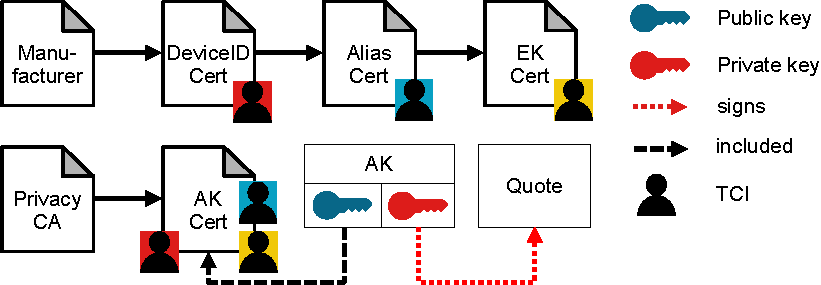
\includegraphics[width=1\linewidth]{figures/privacy-arch.pdf}
  \caption{The adapted architecture integrating privacy.} \label{fig:privacy_arch}
\end{figure}


We also need to transfer the DICE information from the old certificate chain to the new private one.
After performing the formerly described actions, the privacy CA creates a certificate vouching for that the AK was generated by an authentic TPM, hiding which exact TPM, even the manufacturer.
The privacy CA also copies each TCI of the old certificate chain into the AK certificate, as depicted in \autoref{fig:privacy_arch}.
The yielding private certificate chain is returned to the prover, who can forward it to a verifier without revealing its identity.

Whether the verifier trusts the firmware TPM is conducted in the same way as described in \autoref{subsec:trust_prover_tpm}, with the only difference is that the TCIs are all embedded into a single certificate, i.e., the AK certificate.
The verifier must also be able to trust the prover's quote as explained in \autoref{subsec:trust_quote_from_prover}.
For that, the verifier must trust the issuer of the AK certificate to have verified that the \ac{AK} is stored on an authentic TPM\@.
However, the privacy CA does not need to check whether AK is restricted.
This can be carried out by the verifier itself, as it continues to receive the TCI of the fTPM\@.

Ultimately, this adapted privacy architecture changes the statement a verifier can make from ``I am communicating with this authentic TPM in control of this EK'', to ``I am communicating with some authentic TPM in control of this AK.''
In other words, the verifier does not know exactly which TPM they are communicating with.
The privacy of the prover is guaranteed by the fact that the prover does not transmit any data derived from its \ac{UDS} to the verifier.

Nevertheless, privacy is not fully ensured because of the TCI values revealed to the verifier.
The order and values of the TCIs of an AK certificate might be sufficient to identify that it communicated with this particular prover before.
This can only be prevented by transferring the evaluation of the TCIs from the verifier to another entity, e.g., the privacy CA\@.
One possible realization is for the privacy CA to add to its policy that it will only certify AKs if they originate from a prover it considers trustworthy based on the TCIs it provided.
However, this makes the verifier dependent on another entity that decides whether the TCIs provided are trustworthy or not, which we consider undesirable.

We also want to highlight that the AK does not need to be a child of the EK, it does not even have to be part of the endorsement hierarchy.
In fact, it should not be part of the endorsement or platform hierarchy, since the TPM behaves differently when signing a quote depending on the hierarchy of the signing key~\cite{tpm20}.
If the signing key is part of the endorsement or platform hierarchy, the TPM assumes that privacy is irrelevant and embeds the TPM's firmware version, reset count, and restart count in plaintext in its generated quote.
This tuple might identify the TPM\@.
If the key is part of another hierarchy, this data is obfuscated by adding random offsets to each value, which is desirable if privacy is a concern.

% TODO: Maybe put somewhere earlier
% In general, endorsement keys represent device identities and are therefore privacy-sensitive.
% Our EK takes on the role of an attestation key, which has the task of signing attestation evidences.
% Although our EK does not represent the device identity, it does represent the identity of the shorter lived fTPM.
% This makes our EK also privacy-sensitive, since its generated signatures can be cross-referenced and then traced back to the according EK.
% Our approach has the advantage that we do not need a trusted third party, but trust the manufacturer of our trust anchor directly (DICE).
% In \autoref{sec:privacy}, an extension of our system is presented with privacy in mind.
